%\documentclass[11pt]{report}
%\usepackage{siunitx}
%\usepackage{graphicx}

%\begin{document}
%\tableofcontents


\newpage
\chapter{Introduction}
This chapter introduces the underlying concepts and main goals behind Tissue Engineering (TE) research. \ac{TE} variability sources are introduced, a critical context scarcely addressed, which motivated this thesis work. An overview of the thesis subject and main goals is exposed, where \ac{BTE} is presented as a subset of tissue engineering recursively targeted as a proof of concept along the developed work.


\newpage
\section{Tissue Engineering strategies}

\ac{TE} is an interdisciplinary field that combines engineering and life sciences research to develop biological substitutes that restore, maintain, or improve the function of an entire organ or tissue. \ac{TE} is pointed out as a desirable solution to be adopted when tissues or organs have been severely diseased or lost by cancer, congenital anomaly or trauma. In those scenarios, conventional approaches are no longer applicable, and the treatment is reduced to the possibility of organ transplantation, often hindered by the shortage of donated organs and immune rejection reactions \cite{Chandra2020-ay}. Over the years, these limitations have led to several attempts to create artificial organs and regenerative medicine approaches, and despite having achieved remarkable scientific advances, they still require improved biocompatibility and functionality \cite{Ikada2006-cd}. \ac{TE} applications can be categorized into scaffold-based and scaffold-free approaches, considering the need to add extracellular matrices to fill a tissue/organ defect, while providing structural support and a fixation area for native or implanted cells. In a bird’s-eye view, a \ac{TE} approach for healing an organ defect consists of a sequence of procedures, as illustrated in Figure \ref{fig1d1}. This approach starts with obtaining an undifferentiated cell line from an autologous biopsy or an allogenic compatible donor. This initial cell line is commonly isolated and proliferated in a static culture until it reaches confluence. Then, cell culture procedures are applied accordingly with the \ac{TE} strategy selected, scaffold-free versus scaffold-based. Their overall distinction and major techniques are introduced in subsequent subsections, considering that both pretend to achieve the same goal of repairing the original organ defect.  


\begin{figure}
\makebox[\textwidth][c]{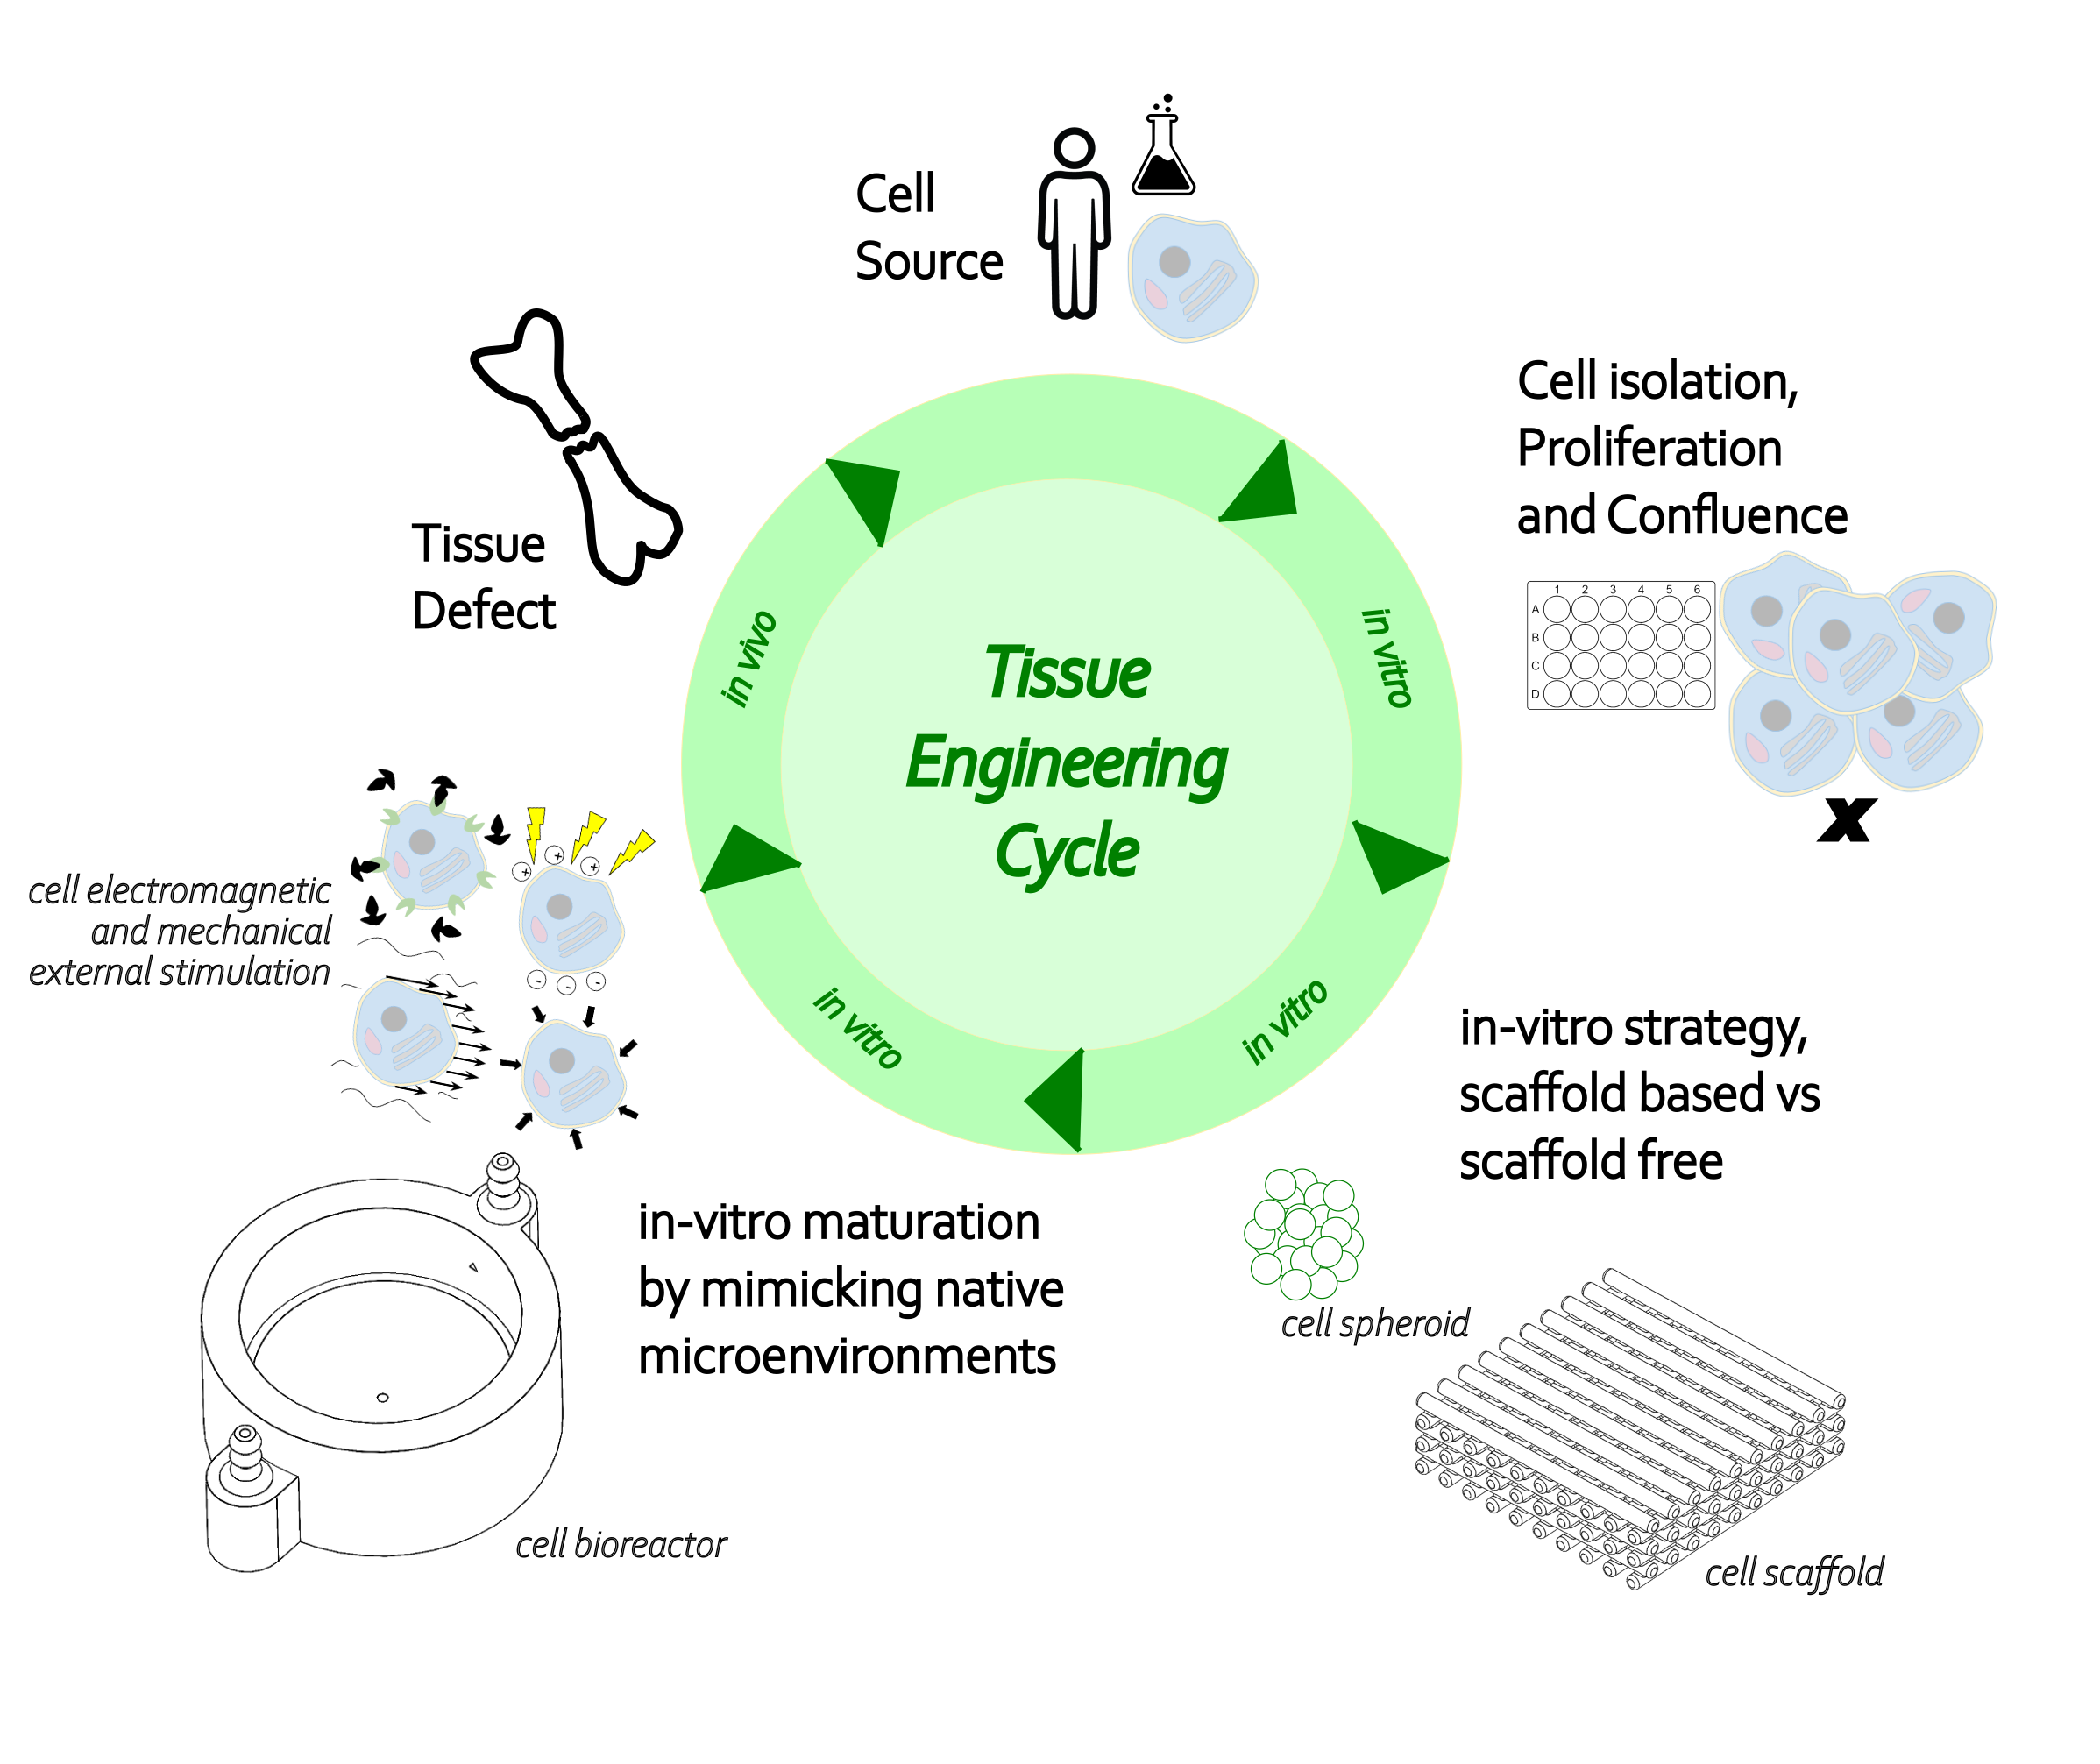
\includegraphics[scale=0.25]{./figures/Figure_1d1.png}}
\caption{The tissue engineering cycle: illustration of the main steps involved.}
\label{fig1d1}
\end{figure}


\subsection{Scaffold-free strategies}

Scaffold-free strategies are characterized by not using cell seeding or adherence within an exogenous material, which will require large cell numbers to secrete even more significant amounts of \ac{ECM} \cite{DuRaine2015-fu}. This bottom-up strategy seeks to produce tissues by mimicking developmental processes following this pattern: cell condensation, cell proliferation, cell differentiation, \ac{ECM} production, and tissue maturation. Scaffold-free approaches account for self-organization or self-assembly events at the cellular level to obtain sheets, spheroids, or tissue strands as building blocks. This strategy's success relies on these building blocks' capacity to secrete a favorable extracellular matrix fusing into larger tissue constructs \cite{Dissanayaka2020-ig}. Cell sheet engineering is one of these scaffold-free techniques where cells are expanded in a monolayer until they achieve a high confluence. Once a cohesive \ac{ECM} layer is obtained, the resultant sheet is lifted and externally manipulated to form the desired structure. Also, multiple sheets can undergo tissue fusion to address more extensive tissue defects \cite{DuRaine2015-fu}. Aggregate tissue engineering is another scaffold-free technique that uses self-organized cell aggregates (cell spheroids) that occur in culture, by applying a rotational force or another non-adherent process to cells in a suspension. Fusing small aggregates to form larger tissues, or injecting aggregates into defects, are considered two of the most promising methods to apply this technique. A recent development is the deposition of cell aggregates in spheroids and strands as cell-only bio-ink to additively fabricate complex \ac{3D} printed constructs \cite{Khoshnood2020-ll}. Another emergent scaffold-free strategy is simultaneously a cell-free strategy. It selectively isolates a set of paracrine molecules and biological factors, collectively termed secretome, due to being secreted by cells into the extracellular space. This strategy suggests that a significant part of cell-based therapeutic benefits are due to their secretome, which may include extracellular vesicles that, after being collected, are applied to the original organ defect impacting many regenerative biological functions \cite{Daneshmandi2020-nn}.


\subsection{Scaffold-based strategies}

Scaffold-based strategies mainly rely on using biomaterials to create a \ac{3D} structural construct with interconnected pores (the scaffold) that support the seeded cells throughout the process of tissue formation \cite{Dissanayaka2020-ig}. The scaffold and the adherent cells are cultured under appropriate biophysical and biochemical conditions for further proliferation and differentiation into the desired tissue \cite{Howard2008-qk}. \textit{In vitro} cell cultures can be made static or dynamic (inside a bioreactor), a culture option that dictates the availability of nutrients and metabolic waste removal according to the profile of the generated culture media fluid flow. When the cultured tissue reaches maturation, a subsequent transplantation phase is performed to address the original \textit{in vivo} health condition. \ac{TE} scaffolds are designed to influence the physical, chemical, and biological environment surrounding a cell population \cite{Reina-Romo2019-ry}. To do so,
scaffold biomaterial(s) are selected accordingly with the cell(s) type and source to promote their adhesion, proliferation, and differentiation. An extensive list of biomaterials and their correspondent cellular interactions has been compiled for a wide range of different cells \cite{Qu2019-qq}, highlighting those that provide improved support and attachment surface, while simultaneously serving as a platform to deliver chemical and physical environmental cues (e.g., growth factors, surface proteins, cellular signals, electrical or mechanical patterns). It is well established that cell function is influenced by scaffolds' composition, topography, and architecture, along with the presence of soluble mediators sculpt the success of scaffold-based strategies \cite{Ripamonti2004-vm}. The adequation of scaffold properties and design to generate the most favorable environment (\textit{in vitro} or \textit{in vivo})  for tissue regeneration is the current critical challenge in scaffold-based strategies \cite{Hutmacher2023-le}.   


\section{Bone tissue engineering}

\ac{BTE} is a subset of tissue engineering dedicated to provide novel methods to treat segmental and contained skeletal defects difficult to repair by conventional strategies. The main idea is to restore the natural signaling pathways of bone development and heal the existing skeletal defects. The standard approach to bone regeneration in \ac{BTE} includes three building blocks: a cellular osteoblastic line that secretes bone matrix (or its progenitor cell line); a scaffold to support cellular attachment and fill the skeletal defect, providing appropriate mechanical stability; bounded systems capable of triggering osteoinduction through the delivery of osteoconductive signals and growth/differentiation factors. Osteogenesis induction of bone progenitor cell lines usually includes dexamethasone, ascorbic acid and sodium-Beta-glycerophosphate to promote differentiation, and \ac{VEGF}, \ac{FGF} or \ac{BMP} to promote growth \cite{Francois2019-ip, Miron2012-vk, Franz-Odendaal2006-eu}. A recent strategy to obtain bone tissues begins with engineering cartilaginous constructs and then attempts to recapitulate the embryonic processes of endochondral ossification \cite{Fu2021-us}.

There is an increasing demand for \ac{BTE} clinical approaches due to the short donor supply of bone substitutes (bone grafts), following the demographic rise of the elderly population. A systematic analysis conducted worldwide (including 204 countries and territories) from 1990 to 2019 concluded that in 2019, there were 178 million new fractures (a 33.4\% increase since 1990), 455 million prevalent cases of acute or long-term symptoms of a fracture (a 70.1\% increase since 1990), that are translated to 25.8 million years lived with disability (a 65.3\% increase since 1990) \cite{Cauley2021-vt}. This data reflects a significant societal and economic cost. In the European Union, the bone fragility fractures in the six founding member states are estimated to increase 23\%, from 2.7 million in 2017 to 3.3 million in 2030 \cite{Borgstrom2020-ki}. These will be further aggravated as the European 'age quake' approaches its historical highest magnitude, going from a median age of 37.7 years old in 2003 to a median age of 52.3 years old by 2050.

Bone fractures may occur after trauma, infection, or oncologic resection. Minor bone defects usually heal without complex interventions, but critical size defects (incapable of spontaneous healing) require one or more surgical procedures to induce union and regeneration \cite{Gordeladze2017-gs}. These surgical interventions involve bone-grafting techniques and other slow healing techniques with autologous or allograft bone that have the disadvantage of regularly producing problems such as fast degradation rates, reduced bioactivity, donor site morbidity, or the risk of pathogen transmission \cite{Peric_Kacarevic2020-hp}. Another drawback of traditional treatments is that there is no guarantee that the applied procedure can completely correct the bone defect. Therefore, searching for surgical alternatives presents a crucial challenge in orthopedic traumatology \cite{Guerado2017-un}.

Anatomically, bone is composed of two distinct regions, one containing dense and solid cortical bone and the other containing honeycomb-like trabecular cortical bone. Cortical bone accounts for 80\% of the total bone mass and performs the major structural function of bone. In terms of mechanical characteristics, cortical bone possesses a compressive strength ranging from 100 to 230 \si{\mega\pascal} and Young’s modulus ranging from 10 to 20 \si{\giga\pascal}, while trabecular bone only reaches 2–12 \si{\mega\pascal} and 0.01–0.9 \si{\giga\pascal}, respectively \cite{Chang2022-ah}. Microscopically, trabecular bone is unorganized and unstructured, while the cortical bone is composed of spatially organized structures, called osteons. These are identified as a hierarchical cylindrical structure surrounding a Haversian canal containing osteocytes, lamellae, and the lacunocanalicular network. The capability of sensing and transducing mechanical stress is attributed to osteon networks, making the bone responsive to external stimuli, moreover, the Haversian canal is known to transport osteoclast and osteoblast progenitor cells to initiate cortical bone remodeling \cite{Chang2022-ah}. Osteocytes are the key regulator of bone turnover \cite{Goldring2015-kn}, mediating osteoclast bone absorption by modulating the RANKL/OPG expression pattern on the plasma membrane and mediating osteoblast bone formation by releasing DKK-1 and sclerostin, two critical inhibitors of the Wnt/b-catenin pathway. Moreover, osteocytes can indirectly participate in bone turnover by secreting bioactive molecules (e.g., prostanoids, nitric oxide, IGF, VEGF, TGF-b), playing critical roles in mechanosensation that is probable to be activated by sensing the bone fluid flow shear stress within the lacunocanalicular network \cite{Murshid2022-rs}. The detailed mechanism of osteocyte mechanotransduction remains a topic under active discussion, trying to make sense of the particular roles of its dendrites, primary cilia, and cell membrane receptor integrins. Nitric oxide, ATP, and prostaglandin have been proposed as signal mediators in this process \cite{Nguyen2013-bx, Geoghegan2019-qi}.

Bone is a composite tissue with organic (mainly made of collagen type I) and inorganic phases (primarily calcium phosphates in the form of \ac{HA}) \cite{Peric_Kacarevic2020-hp}. Regarding cellular content, the most abundant cellular component of mammalian bone cells is osteocytes, approximately 95\% of all bone cells. There are ten times more osteocytes than osteoblasts in an individual bone \cite{Franz-Odendaal2006-eu}. When a critical size fracture occurs, the standard \ac{BTE} approach is to fill the bone defect gap with a scaffold material that should provide characteristics similar to the previously existing native bone structure, such as surface roughness, porosity, pore size interconnectivity, degradation rate, mechanical properties, and biocompatibility. Osteogenesis will occur on the implanted scaffold, depending on its capability to recruit four primary bone cells: bone-lining cells, osteocytes, osteoclasts, and osteoblasts. A significant focus is given to recruiting osteoblasts since their functions include depositing \ac{HA} crystals into the voids between the collagen fibrils, a process called biomineralization. The degree of biomineralization is the characteristic that determines the mechanical properties of a particular bone tissue. Osteoblasts produce new bone and originate from \ac{MSCs} \cite{Franz-Odendaal2006-eu}. \ac{MSCs} may play a significant role in \ac{BTE} strategies due to their capacity for osteogenic differentiation and their abundant availability, since they exist in many organs and tissues of the human body \cite{Guillot-Ferriols2022-wn}. Regarding bone graft substitutes (\ac{BTE} scaffolds), despite the possibility of being made from different materials (e.g., natural or synthetic polymers, bioceramics, metals), they should provide an osteointegrative, osteoinductive, and osteoconductive environment. The osteoinduction process stimulates immature cells (\ac{MSCs}) to develop into preosteoblasts, a process that is typically conducted \textit{in vitro} inside a bioreactor. This mentioned bioreactor unit is one of the central technologies in \ac{BTE} supporting scaffolds and adherent cells, with the increasing mass transport requirements of growing tissues. The bioreactor also allows a controlled recreation of an osteoinductive cellular environment (e.g., chemically, mechanically, electrically), mimicking bone native conditions until the sustained cell culture is sufficiently mature to be transplanted and fill patients' original bone defect.

This thesis research chose \ac{BTE} with the described scaffold-based strategy as a proof of concept due to its growing relevance and the fact that bone cells naturally respond to mechanical and electrical stimulation \cite{Wang2022-op, Nunez-Toldra2020-ai}. This methodological reductionism, from \ac{TE} to \ac{BTE}, is required for practical demonstration and analysis. Even if some conclusions are only valid for the selected cell/tissue type under study, the subjacent developed systems and techniques can be adapted to apply in other \ac{TE} areas without losing their feasibility.


\section{\textit{In-vitro} experimental variability sources}

The final goal of \ac{BTE} is to repair the patient's bone defect. The success of \ac{BTE} strategies crucially depends on the final \textit{in vivo} reimplantation phase, which conceals many unknown uncertainties in the complex biochemical and biophysical interactions between the implant and target tissues. To achieve a successful \ac{BTE} strategy, one must first make sense of the previous \textit{in vitro} cell culture phase before moving on to implantation. It is known that the state-of-the-art in \ac{BTE} \textit{in vitro} research presents a core problem: high research variability in experimental settings and outcomes. This variability lowers reproducibility and narrows the application of \ac{BTE} outputs into everyday practice. This subchapter focuses on identifying the primary sources of variability in \ac{BTE} research. This is an essential step to determine how \textit{in vitro} outcomes can be controlled to increase reproducibility and finally address the remaining challenges of the \textit{in vivo} phase.

\subsection{Bioreactors, flow regimes, and scaffolds}

To bioengineer a bone graft, it is required to pick an adequate cell source and seed the selected cells in an adequate number into the cell support structure, while at the same time providing all the appropriate \textit{in vitro} cell culture conditions to achieve significant levels of proliferation and differentiation. Many systems have been developed and applied in \ac{BTE} over the years to obtain the living bone grafts described above. Nevertheless, it is the presence of two standard non-biological systems that directly support cell culture: a bioreactor system (see Figure \ref{fig1d2}), defined by the vessel that contains the cell culture, responsible for the control and actuation processes, efficiently performing cell nutrient support, cell waste removal and temperature stabilization; a scaffold system, composed of the biomaterial that provides structural support and a tridimensional orientation for cells to migrate and grow, mimicking \ac{ECM} functions. 

\begin{figure}
\makebox[\textwidth][c]{\includegraphics[scale=0.07]{./figures/Figure_1d2.png}}
\caption{Standard non-biological systems that directly support cell culture are shown to exemplify the diversity of systems that need to be accounted for. Shown bioreactor systems differ in operation, design, and level of automation, constituting a source of \textit{in vitro} experimental variability. Additionally and independently from the bioreactor chosen, multiple cell culture options (listed in the image's top left corner) will impact the cell culture results. All bioreactors present in the figure are perfusion bioreactors adapted from the literature \cite{Lim2019-gx, Birru2018-rj, Gabetti2022-hp}.}
\label{fig1d2}
\end{figure}

Bioreactor technologies in \ac{BTE} can be divided into three categories: perfusion bioreactors, rotating bioreactors, and spinner flask bioreactors \cite{Kazimierczak2022-mq}. Vessel design, construction techniques, and mode of operation pose significant differences between these categories \cite{Melo-Fonseca2023-fd}. Differences also appear when comparing systems inside the same category. Computational modelling studies of media flow in \ac{BTE} reactors revealed different fluid velocity profiles that induce a significant variation in shear stress distribution when comparing results between perfusion with rotating \ac{BTE} bioreactors \cite{Nokhbatolfoghahaei2020-yt}. Since different levels of shear stress are expected to generate different cellular outcomes, bioreactor-dependent velocity profiles constitute an important source of experimental variability. 

Calling for best practices in mammalian cell culture environmental control is becoming prominent \cite{Klein2021-dz, Klein2022-yj}.  Even slight deviations in mammalian cell culture from the physiological levels, regarding \acs{pH} \cite{Michl2019-js} or dissolved gasses (\acs{dO2}, \acs{dCO2}) \cite{Ast2019-mc, Place2017-bn}, can provoke substantial cellular perturbations. This, in turn, can profoundly impact study conclusions when these conditions are incorrectly assumed to be stable, or when a critical biological parameter for reproducibility is ignored and routinely not measured or incorrectly reported \cite{Al-Ani2018-df}. The evolution of bioreactor systems to improve upon these best control practices is critical to increase the understanding of experimental results in \ac{BTE}.

Performing cell cultures on tissue-engineered scaffold structures adds a new group of variability sources. The specific interactions between the seeded cells and the introduced biomaterial structural and physical attributes became relevant to consider \cite{Zaeri2022-wk}. For instance, the presence of a scaffold in the cell culture chamber contributes to different nutrient flow and diffusion patterns emerging from its geometry interference \cite{Woo_Jung2013-yq}. The scaffold fabrication process also plays a role in introducing variability, adding specific limitations and outcomes influenced by the fabrication process itself. For example, scaffolds produced by rapid prototyping techniques show architecture variations compared to the original \ac{CAD} design and intersample variability, when compared to other scaffolds produced by the same fabrication process \cite{Campos_Marin2015-qc}. Computer fluid models were performed on additive-manufactured scaffolds reconstructed by \ac{mCT}. Those \ac{mCT} modelling results revealed different fluid velocity and \ac{WSS} profile patterns, showing higher values and more irregular profiles when compared to the precursor \ac{CAD} model analysis. Also, from sample to sample, different \ac{WSS} patterns emerged. These variations affect local fluid velocities and \ac{WSS} values, affecting each cell's mechanical microenvironment and becoming a noise source for \textit{in vitro} experiments. In the worst-case scenario, they may result in heterogeneous cell distributions and different cell responses throughout the scaffold. Scaffold inspection/verification processes based on \ac{mCT} reconstructions have been proposed to become a standard practice to understand the impact of manufacturing limitations on scaffold geometry and consequent biological performance \cite{Podshivalov2013-sy}. 

\subsection{Cell sources and cell culture options}

From static to dynamic cell cultures, with or without cell support structures, a documented important source of variability are the options adopted regarding cell source and cell culture process. Different cell types or even the same cell type from different origin tissues or cellular phases have different metabolic needs that, without proper care, can deplete the culture medium of nutrients \cite{Al-Ani2018-df}. Oxygen consumption ratios, cell seeding density, experiment duration, culture vessel geometry, and media volume all interplay to influence cell nutrient availability, impacting cell culture outcomes. This is even more complex if we consider, for example, that a  proper oxygen delivery must account for additional parameters affecting solubility like temperature variations, atmospheric partial pressure, humidity, carbon dioxide concentration, convective mixing systems, and the ionic strength of culture media, all affecting the amount of oxygen available to cells at each moment. Also, practices for handling the tissue culture should be carefully considered since the number of times they are handled, and the handling procedure exposes the cell culture to different gas mixtures, causing changes in the oxygen concentration in the culture media. Those changes may provoke an imbalance that can take hours to reach a new equilibrium steady state.

Focusing on cell growth and avoiding apoptosis, good cell culture media selection allows controlling osmolality, ammonia levels, and the production of free radicals \cite{Price2017-mm}. For optimal results, researchers need to know the best physical parameters of the cells intended to be cultured. Those will allow supplying: an adequate balanced salt solution in terms of concentrations of anions (e.g., PO\textsubscript{4}\textsuperscript{3-}, Cl\textsuperscript{-}, HCO\textsubscript{3}\textsuperscript{-}) and cations (i.e. Na\textsuperscript{+}, K\textsuperscript{+}, Ca\textsuperscript{2+}, Mg\textsuperscript{2+}); proper levels of energy sources (i.e. glucose and glutamine), vitamins, essential and nonessential amino acids, lipids. The optimal choice of medium depends on the target cells and the purpose of the research. Choosing between classical formulations with serum, serum-free options, or chemically defined media has advantages and disadvantages. Insufficient nutrients or excess toxic byproducts will profoundly impact cell culture results. A significant cause of lack of reproducibility in \ac{TE} applications is the poor implementation of quality control measures and reporting standards. For this reason, good cell culture practices and guidelines for every process step are constantly being updated and revised \cite{Pamies2018-fm, Geraghty2014-rb, Pamies2022-cq}.

\subsection{External stimulation technologies and protocol options}

Mechanical and electromagnetic stimuli have been routinely added to the existing cell culture conditions through specially designed external stimulation systems to lead cells into improved proliferation or/and differentiation or to mimic native tissue conditions where they naturally exist.  

In BTE, fracture healing is a complex, multistep process susceptible to mechanical signaling and micro-mechanical cues \cite{Anani2022-vm}. External mechanical stimulation systems vary in their core technology; by doing so, they all deliver mechanical stimuli with slightly different characteristics. The use of low-intensity pulsed ultrasound, for example, applies an oscillating longitudinal pressure wave with a frequency generally greater than 20 kHz \cite{Harrison2021-gy}. Other techniques use a constant or sinusoidal applied hydrostatic pressure (waveform from 0.001 to 2 Hz) \cite{Henstock2013-co, Nesler2016-le, Stavenschi2018-ze}, whose magnitude is reported to vary between 0 and 300 kPa. More standard methods to apply mechanical stimuli involve direct compression/elongation of the scaffold structure or resorting to perfusion interactions, like fluid flow-induced wall shear stress, to transmit forces to the seeded cell region \cite{Wittkowske2016-xr}. This multitude of methodologies resulted in a significant number of designs that can be generally categorized as fluid perfusion systems, rotary devices (e.g., spinner flasks), dynamic compression/tension systems, vibrational and hydrostatic pressure chambers \cite{McCoy2010-hy, Sart2016-uq, Campsie2019-jq}. These different systems and their multiple protocols introduce specific differences in the cellular microenvironment generated by mechanical stimulation and consequent mechanotransduction effects. This hinders the comparison among results to retrieve solid conclusions \cite{Sun2022-xt}.

Electromagnetic field stimulation in BTE has been shown to promote different ranges of cellular response, from proliferation, migration, growth, differentiation, extracellular matrix expression, or even apoptosis \cite{Thrivikraman2018-su}. Electric fields (\acs{EFs}) are thought to transiently change membrane polarization and permeability of specific ion channels, modulating cascades of events at the intracellular level \cite{Bhavsar2019-iz}. The application of an electromagnetic field consists of a non-specific process that targets any charged particle. Thus, various cellular processes may be modulated by \acs{EFs} with different characteristics (e.g., different magnitudes and frequencies). Experimental setups that apply electromagnetic fields are commonly classified into three groups \cite{Thrivikraman2018-su, Balint2013-rd, Nicksic2022-jy}: 

\begin{itemize}
\item \ac{CCoupled} systems - these apply a time-varying electric field, with both setup electrodes separated from the cell culture medium by an electric insulator layer. A less used variant is the Semi-Capacitively Coupled system, where one of the electrodes is in direct contact with the cell culture medium while the other remains electrically insulated;

\item \ac{DCoupled} systems - a steady or time-varying electric field is applied, with both setup electrodes in contact with the cell culture medium (immersed), or separated from the cell culture medium by an agar-salt bridge;

\item \ac{ICoupled} systems - the setup usually comprises Helmholtz coils that apply a time-varying magnetic field, producing an induced electric field in the cell culture medium region (electromagnetic induction).
\end{itemize}

\ac{ICoupled} systems contrast with the other groups because they apply electromagnetic stimulation by delivering superimposed electric and magnetic fields. An exception can be made to \ac{ICoupled} applications like the transformer-like coupling method, which allows to isolate cellular effects due only to an \ac{EF} \cite{Hess2012-kw}. Even though \ac{CCoupled} setups had less expression in recent publications relative to \ac{DCoupled} and \ac{ICoupled} configurations, this kind of setup offers some advantages when trying to minimize experimental variability. First, \ac{CCoupled} electrodes are not in direct contact with the culture medium, contributing to block electron transfer to the culture medium, avoiding the formation of oxidative radicals species (faradaic products), usually present in \ac{DCoupled} setups, and whom may influence cellular response and survival \cite{Srirussamee2021-cj}. Second, \ac{CCoupled} devices allow to isolate the effects of the \acs{EFs} without additional chemical artifacts, a feature also achievable in ICoupled setups, but with no distinction between actions of electric and magnetic fields. Besides the technology differences, high protocol dissonance can be observed and is extensively compiled in literature reviews \cite{Kim2015-vg, Ryan2021-tq, Da_Silva2020-su, Thrivikraman2018-su}. The mentioned reviews state that difficulties in concluding electrical stimulation studies mainly arise from the varying values of applied stimulation strength or other differences in stimulation protocols, aggravated by incomplete device specification. Thus, it is recommended to increase scientific rigor and report a novel minimum set of parameters \cite{Nicksic2022-jy}.
 
Figure \ref{fig: F3} establishes a visual comparison between a sample of protocols applied in \ac{DCoupled} \acs{EFs} stimulation to exemplify the substantial variability between different experimental studies, even when considering the same external stimulation technology and cellular line.

\begin{figure}
\makebox[\textwidth][c]{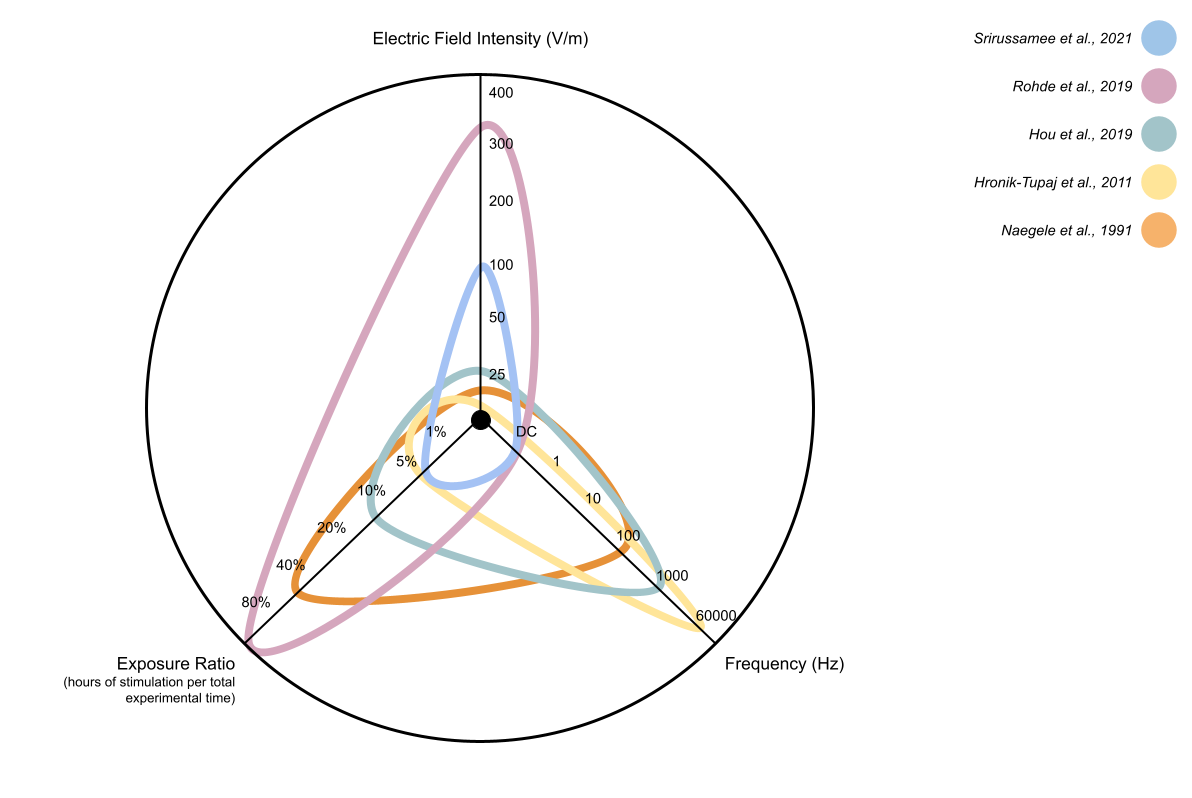
\includegraphics[scale=0.4]{./figures/Figure_1d3.png}}
\caption{Protocol design variability in electromagnetic field stimulation parameters, considering five different \ac{DCoupled} \acs{EFs} studies \cite{Srirussamee2021-cj, Hou2019-yd, Hronik-Tupaj2011-cx, Zhao2011-wy}.}
\label{fig: F3}
\end{figure} 


\section{Context of the thesis}

In TE and BTE, bioreactor and scaffold design are of paramount importance to promote and sustain adequate \textit{in vitro} conditions for cell culture differentiation, proliferation, growth, and support. In addition to nutrient transport and waste removal, diverse bioreactor designs have been developed to provide mechanical or electromagnetic stimuli to cells, enhancing physical microenvironmental conditions to unlock specific cell responses. Previous studies have shown that single or combined stimuli significantly upregulate important cellular functions related to regenerative processes. For different stimulation types and cellular tissues, adequate stimulation properties have been experimentally determined and reported in several \textit{in vitro} studies. However, the biophysical mechanisms by which cells sense, interpret, and transform these stimuli into actions remain unclear. Even under the same cellular lines, experimental protocols present a high variability (quantitative and qualitative) of stimulation parameters and also on the geometry and materials of the setup used for applying the intended stimuli. Reported results of diverse stimuli application prove to have beneficial effects in cell cultures. Still, their protocol design variability originates questions regarding the most appropriate and relevant stimulation parameters and which effects are being effectively produced and observed \cite{Thrivikraman2018-su}.

This Ph.D. thesis aims to develop a multimodal stimulation all-in-one bioreactor design strategy attempting to combine electromagnetic and mechanical stimulation under a common open-source platform. This concept includes sensors for online monitoring and control units to fully automate the bioreactor system. The process of designing the intended bioreactor also includes scaffold design stages, both of them guided by their digital model (an accurate virtual numerical model constructed to reflect the physical object). These constructed numerical models allow us to precisely predict the delivered biophysical microenvironment, a piece of information useful to optimize the bioreactor and scaffold in the design phase. These models are also useful to redefine stimulation protocol standards for bone cell stimulation, fine-tuning the stimulation to better test and provoke cellular responses. Additionally, this thesis proposes a data-driven design methodology based on numerical model predictions, to better understand the underlying biophysics of external stimulation systems and the impact of adding scaffold structures to the cell culture chamber in stimulation-induced outcomes. Despite making the analysis in the subset of \ac{BTE}, most of the conclusions can be easily transferred to other tissues, opening new perspectives for stimulation systems in \ac{TE}. An open-science commitment is made in this thesis, through sharing of detailed methodologies and results in open-source public repositories. This contributes to increase shareability, reproducibility, and standardization of \textit{in vitro} stimulation and culture experimental procedures among researchers.

\subsection{Thesis overview}
This thesis is organized as follows:
\begin{itemize}
\item Chapter 1: Introduction;
\item Chapter 2: Numerical models of external stimulation methods;
\item Chapter 3: Numerical modelling of mechanical stimulation;
\item Chapter 4: Numerical modelling of direct-coupled electric field stimulation;
\item Chapter 5: Numerical modelling of capacitive-coupled electric field stimulation;
\item Chapter 6: All-in-one bioreactor design methodology driven by numerical model predictions;
\item Chapter 7: Final considerations;
\item Chapter 8: Scientific outputs.
\end{itemize}


%\newpage
%\bibliography{library_c1} 
%\bibliographystyle{plain}
%\end{document}